\documentclass[11pt,a4paper,twoside]{report}
\usepackage{amsmath,titlesec}
\usepackage{paralist}
\usepackage[scaled]{beramono}
\usepackage{colortbl}
\definecolor{gray-5}{gray}{0.95}
\definecolor{gray-10}{gray}{0.9}
\definecolor{gray-20}{gray}{0.8}
\definecolor{gray-30}{gray}{0.7}
\definecolor{gray-40}{gray}{0.6}
\definecolor{fadered}{rgb}{0.988, 0.914, 0.310}
\usepackage{charter}
\usepackage{longtable}
\usepackage{multirow}
\usepackage{multicol}
\usepackage[pdftex]{graphicx}
\usepackage{caption}
\usepackage[top=1in, bottom=1in, left=1in, right=1in]{geometry}
\usepackage[charter]{mathdesign}
\usepackage[utf8]{inputenc}
% \usepackage[none]{hyphenat} 
\usepackage{natbib}
\usepackage{float}
\usepackage[final]{pdfpages}

\usepackage{sidecap}

\makeatletter
  \newenvironment{SCtopfig}{\SC@float[t]{figure}}{\endSC@float}
\makeatother

% \usepackage{setspace}
\usepackage[charter]{mathdesign}
% \usepackage[small]{caption}
% \usepackage{abstract}
% \usepackage{lineno}
\setlength{\headheight}{14pt}
% \newcommand{\includepublication}[1]{\includepdf{#1}}
\newcommand{\includepublication}[1]{}
\usepackage{nomencl}
\makenomenclature

\sloppy

\usepackage{listings} 
\lstset{numbers=left, numberstyle=\scriptsize\ttfamily, numbersep=10pt, captionpos=b} 
\lstset{backgroundcolor=\color{gray-5}}
\lstset{basicstyle=\small\ttfamily}
\lstset{framesep=4pt}
\lstset{language={}}
\newcommand{\inlineCode}{\lstinline[basicstyle=\normalsize\ttfamily]}
\newcommand{\first}[1]{{\vspace{1ex}}{\Large \textbf{#1}}{\vspace{1ex}}}
\newcommand{\second}[1]{{\vspace{1ex}}{\large \textbf{#1}}}
\newcommand{\tabspace}[0]{\vspace{2mm}}
\newcommand{\cvsubheader}[1]{\multicolumn{2}{@{}l}{\second{#1}} \\ \nopagebreak[4]}
\newcommand{\cvitem}[1]{\input{../../common/#1}}
\newcommand{\cvtitle}[2]{#1 & \textbf{#2} \\ \nopagebreak}
\renewcommand\bibname{References}

\usepackage[colorlinks=true,linkcolor=black,citecolor=black,urlcolor=black,filecolor=black,bookmarks=true]{hyperref}
\hypersetup{
pdfauthor = {Michael Specht},
pdftitle = {},
pdfsubject = {},
pdfkeywords = {},
pdfcreator = {LaTeX},
pdfproducer = {pdflatex}}

% \include{styles/chapterleft}
\include{styles/misc}

\usepackage{setspace}
\usepackage{fancyhdr}
\usepackage{wrapfig}
% \renewcommand{\chaptermark}[1]{\markleft{#1}{}}
% \renewcommand{\sectionmark}[1]{\markright{#1}{}}
% \fancyhead[C]{\rightmark}
% \renewcommand{\headrulewidth}{0pt}
% \renewcommand{\footrulewidth}{0pt}
\def \cre{{\em C.~reinhardtii}}
\def \dmel{{\em D.~melanogaster}}
\def \chlre{{\em Chlamydomonas reinhardtii}}

\def \fmfour{FM4}
\def \augno{AUGUSTUS}
\def \augyes{AUGUSTUS/GPF}
\def \etal{{\em et al.}}
\def \denovo{{\em de novo}}
\def \insilico{{\em in silico}}
\def \mz{{\em m/z}}
\newcommand\caret{\mathbin{\char`\^}}

\hyphenation{AUGUSTUS}
\hyphenation{chro-ma-to-gra-phy}
\setlength{\parskip}{2mm}
\setlength{\parindent}{0mm}
\renewcommand{\baselinestretch}{1.4} 
\renewcommand{\arraystretch}{1.4} 

\renewcommand{\headrulewidth}{0.25pt}

% \pagestyle{fancy}

%\setlength{\marginparwidth}{1.5cm}
%\newcommand{\note}[1]{\marginpar{\color{gray-40}\footnotesize \flushleft #1}}
\newcommand{\note}[1]{}

\newcommand{\imageCourtesy}[2]{Image courtesy of #1 \cite{#2}.}

\lstnewenvironment{todo}{\lstset{numbers=none,frame=none,backgroundcolor=\color{fadered}}}{}
% \pagestyle{empty}

% Code for creating empty pages
% No headers on empty pages before new chapter
% \makeatletter
% \def\cleardoublepage{\clearpage\if@twoside \ifodd\c@page\else
%     \hbox{}
%     \thispagestyle{plain}
%     \newpage
%     \if@twocolumn\hbox{}\newpage\fi\fi\fi}
% \makeatother \clearpage{\pagestyle{plain}\cleardoublepage}


\renewcommand{\headrulewidth}{0.25pt}
\fancyhf{}
\fancyhead[EL,OR]{\thepage}
\renewcommand{\chaptermark}[1]{\markboth{#1}{}}
\renewcommand{\sectionmark}[1]{\markright{#1}}

\fancypagestyle{plain} {
    \renewcommand{\headrulewidth}{0.0pt}
    \fancyhf{}
    % \fancyhead[ER]{\leftmark}
    % \fancyhead[OL]{\rightmark}
}


% Code for creating empty pages
% No headers on empty pages before new chapter
\makeatletter
\def\cleardoublepage{\clearpage\if@twoside \ifodd\c@page\else
    \hbox{}
    \thispagestyle{plain}
    \newpage
    \if@twocolumn\hbox{}\newpage\fi\fi\fi}
\makeatother \clearpage{\pagestyle{plain}\cleardoublepage}

\begin{document}
\pagestyle{empty}
% \pagewiselinenumbers

\includepdfset{pages=-,noautoscale}

\begin{center}
\includegraphics[width=0.5\textwidth]{figures/wwu-logo-black.jpg}

{\Large Institut f\"ur Biologie und Biotechnologie der Pflanzen}

\vspace*{5cm}

% {\bf \Huge {\em Chlamydomonas reinhardtii} from the computational proteomics perspective}
{\bf \Huge Novel high-throughput data analysis strategies in computational proteomics and proteogenomics}

\vspace*{4cm}

{\Large Inaugural-Dissertation zur Erlangung des Doktorgrades der
Naturwissenschaften im Fachbereich Biologie der
Mathematisch-Naturwissenschaftlichen Fakult\"at der
\mbox{Westf\"alischen Wilhelms-Universit\"at M\"unster}}

\vspace*{2cm}

{\Large vorgelegt von}

{\LARGE \bf Michael Specht}

{\Large aus Magdeburg}

{\LARGE April 2011}

\end{center}

\cleardoublepage

\vspace*{550pt}

Dekan: Prof. Dr. Christian Kl\"ambt \newline
Erster Gutachter: Prof. Dr. Michael Hippler \newline
Zweite Gutachterin: Prof. Dr. Simone K\"onig \newline
Tag der m\"undlichen Pr\"ufung: \newline
Tag der Promotion: \newline

\cleardoublepage

\vspace*{200pt}
\begin{flushright}
{\Large\em
To my family, the great life amplifier: \\
Jule, Charlotte \& Leo
}
\end{flushright}

% \clearpage

% \begin{abstract}
% This is the abstract. Lots of hacking and MS here.
% \end{abstract}

% {\bf Abbreviations and acronyms used in the report:}
% 
% DSCAM -- down syndrome cell adhesion molecule, 
% FDR -- false discovery rate, 
% GPF -- Genomic Peptide Finder, 
% MS -- mass spectrometry,
% MS/MS -- tandem mass spectrometry,
% PSM -- peptide/spectral match

% \fancypagestyle{plain}{
% \fancyhf{}
% \renewcommand{\headrulewidth}{0.25pt}
% % \renewcommand{\footrulewidth}{0.5pt}
% \fancyfoot[EL,OR]{\thepage}
% \fancyhead[EL]{\leftmark}
% \fancyhead[OR]{\rightmark}
% }

\cleardoublepage
% \begin{multicols}{2}
\setlength{\nomlabelwidth}{0.15\hsize}
\printnomenclature
% \end{multicols}

\cleardoublepage

\setcounter{tocdepth}{1}
\setcounter{secnumdepth}{1}
\tableofcontents

\clearpage



\nomenclature{2D-PAGE}{two-dimensional polyacrylamide gel electrophoresis}
\nomenclature{AMT}{accurate mass/time}
\nomenclature{CID}{collision-induced dissociation}
\nomenclature{CLI}{command-line interface}
\nomenclature{DIGE}{difference gel electrophoresis}
\nomenclature{DNA}{deoxyribonucleic acid}
\nomenclature{ESI}{electrospray ionization}
\nomenclature{EST}{expressed sequence tag}
\nomenclature{FDR}{false discovery rate}
\nomenclature{FT-ICR}{Fourier transform ion cyclotron resonance}
\nomenclature{GPF}{Genomic Peptide Finder}
\nomenclature{GUI}{graphical user interface}
\nomenclature{HPLC}{high performance liquid chromatography}
\nomenclature{ICAT}{isotope-coded affinity tag}
\nomenclature{iTRAQ}{isobaric tag for relative and absolute quantitation}
\nomenclature{LC}{liquid chromatography}
\nomenclature{MALDI}{matrix-assisted laser desorption/ionization}
\nomenclature{MS}{mass spectrometry}
\nomenclature{MS/MS}{tandem mass spectrometry}
\nomenclature{OMSSA}{Open mass spectrometry search algorithm}
\nomenclature{PSM}{peptide/spectral match}
\nomenclature{PTM}{post-translational modification}
\nomenclature{RNA}{ribonucleic acid}
\nomenclature{RPC}{reverse phase chromatography}
\nomenclature{SCX}{strong cation exchange}
\nomenclature{SDS-PAGE}{sodium dodecyl sulfate polyacrylamide gel electrophoresis}
\nomenclature{TOF}{time of flight}

\clearpage

\pagestyle{fancy}
\renewcommand{\headrulewidth}{0.25pt}
\fancyhf{}
\fancyhead[EL,OR]{\thepage}
% \fancyhead[ER]{\leftmark}
% \fancyhead[OL]{\rightmark}
\renewcommand{\chaptermark}[1]{\markboth{#1}{}}
\renewcommand{\sectionmark}[1]{\markright{#1}}

\fancypagestyle{plain} {
    \renewcommand{\headrulewidth}{0.25pt}
    \fancyhf{}
    \fancyhead[EL,OR]{\thepage}
    % \fancyhead[ER]{\leftmark}
    % \fancyhead[OL]{\rightmark}
}

\cleardoublepage
% ==============================================================
\chapter{Introduction}
% ==============================================================

The availability of genome sequences is a key prerequisite for modern 
biological research.
Even before the discovery of the DNA double-helix structure by 
\citeauthor{Watson1953} in \citeyear{Watson1953}, the gene had for several 
decades been regarded as the central unit representing a 
`hereditary characteristic' \citep{Vries1889} and therefore was considered
to play a major role in elucidating one of the biggest mysteries of nature, 
life itself.
After \citeauthor{Jou1972} published the first bacteriophagic nucleotide 
sequence for a single gene in \citeyear{Jou1972}, more elaborate genome 
sequencing techniques have been developed and refined in the following years
\citep{Gilbert1973, Sanger1975, Maxam1977}, culminating in the publication of 
the full human genome sequence in 2001 \citep{Venter2001}.
The possibility to obtain genome sequences has added considerable momentum
to biological research and full genome sequences for more than 180 species
are available (\cite{Yates2009}, see Table \ref{tab:genome-sizes}).
Aside from the ambiguities introduced by non-coding regions in the genome 
\citep{Gilbert1978} and alternative splicing of genes \citep{Black2003}, 
the genome provides, in theory, all necessary information about which proteins 
can potentially be expressed in a cell.
However, in order to study the dynamic nature of a cell or organism, as for 
example in response to changing environmental conditions, the static information
provided by the genome is not sufficient. 
Consequently, the field of genomics has spurred a number of {\em omics}-related 
areas of research \citep{Sauer2007}.

\begin{table}
\begin{tabular}{|l|r|r|l|}
\hline
Species & Genome size & Predicted genes & Reference \\
\hline
{\em Escherischia coli} & 5.2 Mbp & 5,379 & \cite{Welch2002} \\
{\em Thalassiosira pseudonana} & 34.5 Mbp & 11,242 & \cite{Armbrust2004} \\
{\em Arabidopsis thaliana} & 119 Mbp & 25,498 & \cite{Arabidopsis2000} \\
{\em Chlamydomonas reinhardtii} & 121 Mbp & 15,143 & \cite{Merchant2007} \\
{\em Drosophila melanogaster} & 165 Mbp & 13,600 & \cite{Adams2000} \\
{\em Daphnia pulex} & 200 Mbp & 30,907 & \cite{Colbourne2011} \\
{\em Homo sapiens} & 3.2 Gbp & 20,251 & \cite{Venter2001} \\
\hline
\end{tabular}
\caption{{\bf Genome sizes of selected species.} The range of known genome sizes 
    comprises several orders of magnitude, while the number of genes seems
    relatively unaffected by the genome size.
}
\label{tab:genome-sizes}
\end{table}

\section{Omics-related areas of research}

One such research area, {\em transcriptomics}, deals with the transcription
of genes, as recorded in the DNA, to mRNA.
The transcriptome provides information about gene expression at the mRNA level. 
DNA microarray techniques can be employed to screen the regulation of many
genes in parallel on the transcript level \citep{Schena1995}.
Complementing transcriptomics, the field of {\em proteomics} deals with the total
set of proteins expressed in a cell, tissue, or organism, at a defined time
point and under certain conditions \citep{Yarmush2002, Yates2009}.
The notion of the {\em proteome} was coined by Marc Wilkins in 1994 
to reflect the entire set of proteins that are encoded in a genome and are 
actually expressed by a cell \citep{Wilkins2009}.
The transcriptome can be regarded as a precursor of the proteome.
However, transcriptional regulation does not necessarily correlate to
protein expression in a linear fashion \citep{Rogers2008}.
It is therefore vital to combine various types of qualitative of quantitative
information, including the transcriptome and proteome, with further aspects such 
as evolution and the modeling of interactions on the levels of molecules, 
proteins, and cells to achieve a comprehensive understanding of life.
In the past few years, this approach has manifested itself as {\em systems 
biology} \citep{Vidal2009}.
In addition to genomics, transcriptomics, and proteomics, further fields 
involved in the holistic approach of systems biology include metabolomics,
in which the end-products of metabolic processes are analyzed 
\citep{Daviss2005}.
Furthermore, glycomics and lipidomics which provide a view on life from the
perspective of carbohydrates and lipids, respectively, contribute to the
overall picture in the systems biology framework.

\section{Proteomics}

The central aspects of proteomics are the identification of proteins, 
the identifcation of post-translational modifications (PTM), 
relative and absolute protein quantitation, protein localization, and
protein-protein interaction studies.
An important aspect about the proteome is that it is highly variable and
subject to change over time and changing environmental conditions.
In contrast to the genome and the transcriptome, the proteome most accurately
reflects the phenotype of a cell.
While information provided by genomics acts as a foundation to the possible
expression of a protein by the presence of its respective gene in the DNA,
transcript profiling yields information about gene transcription to mRNA.
However, actual protein abundance is not directly related to mRNA abundance.
mRNA molecules may be subject to rapid degradation, and it is also known that 
mRNA is sometimes not translated into a protein at all \citep{Eddy2001}.
Furthermore, the final function of a protein is heavily influenced by
post-translational modifications such as phosphorylation \citep{Olsen2006} 
and ubiquitination.
Finally, not all proteins are expressed in all cell types or cell compartments,
adding another level of ambiguity.
For these reasons, proteomics is a highly complex research area, requiring
sophisticated techniques to produce confident results in the face of
massive complexity.

\section{Mass spectrometry}

Mass spectrometry provides an excellent means for proteome analysis
\citep{Aebersold2003}, with speed, accuracy, and sensivity rapidly increasing
within the past two decades.
The major goals of mass spectrometry-based proteomics are protein 
identification and quantitation.
However, since most proteins are too heavy to be measured directly, the
analysis is usually performed on the peptide level, with proteins being digested
prior to the measurement using proteolytic enzymes such as Trypsin, Lys-C, or 
Pepsin. 
The inherent ambiguity introduced by protein isoforms or alternative splicing
poses an additional challenge when peptide identifications are shifted to
the protein level.
In addition to the raw amino acid sequence encoded by a gene, post-translational
modifications play an important role in defining the actual function of a
protein.
Post-translational modifications may modify a protein by adding an enzyme or by
chemically modifying certain residues.
Furthermore, structural adjustments such as the formation of disulfide 
bonds between Cysteine residues may be required for the protein to become 
functional.
Employing mass spectrometry, it is possible not only to identify peptides and
proteins, but also to study their various modifications.
Another application of mass spectrometry-based analysis is the localization of
proteins to certain compartments of a cell, for example by semi-quantitative
analysis.

Although modern mass spectrometers are very sensitive, a couple of sample 
preparation steps must be carried out in order to achieve comprehensive 
proteome coverage. 
An example of a mass spectrometry-based proteomics workflow for peptide 
and protein identification is depicted in Fig.~\ref{fig:proteomics-overview}.

\begin{figure}
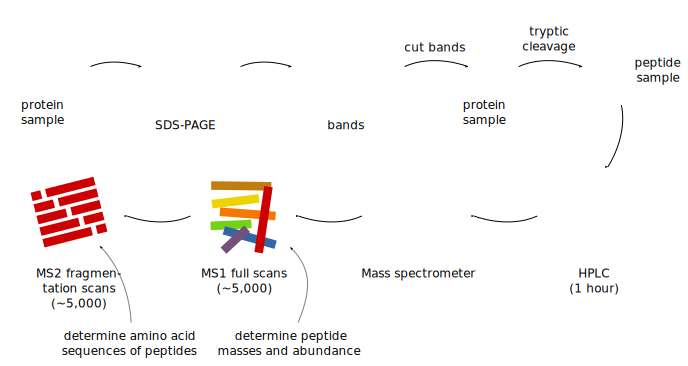
\includegraphics[width=\textwidth]{figures/Proteomics.jpg}
\caption{
{\bf Example of a mass spectrometry-based proteomics experiment workflow.} 
Protein samples are fractionated via SDS-PAGE and resulting bands are excised and
digested proteolytically. In order to further separate the complex mixture, 
the resulting peptides are loaded onto a HPLC column and subsequently eluted 
and injected into the mass spectrometer. Full scans and fragmentation scans
are recorded as peptide elution is in progress for a pre-defined amount of time.
}
\label{fig:proteomics-overview}
\end{figure}

% --------------------------------------------------------------
\subsection{Acquisition of mass spectrometric data}
% --------------------------------------------------------------

Using mass spectrometry, the determination of molecule masses requires 
ionization.
Therefore, values reported in mass spectra are not masses but mass-to-charge 
ratios ({\em m/z}, see Fig.~\ref{fig:mz}).
In the following, the steps involved in the acquisition of mass spectrometric
data are described.

\subsubsection{Preprocessing of biological samples}

% \begin{wrapfigure}{r}{0.6\textwidth}
\begin{SCtopfig}
\centering
\includegraphics[width=0.7\textwidth]{figures/mz.jpg}
\caption{
{\bf Calculation of {\em m/z} values.}
A single peptide may give rise to multiple {\em m/z} values in a mass spectrum,
    depending on its charge. In this example, a singly and doubly protonated
    peptide is shown.
} 
\label{fig:mz}
\end{SCtopfig}
% \end{wrapfigure}

Although mass spectrometric analysis of intact proteins has been successfully
reported \citep{Lee2002, Taylor2003}, such an approach is not feasible in 
general because the high mass of proteins cannot be accounted for with most
types of mass spectrometers.
In addition, low abundant proteins may be missed in complex samples due to
the fact that there are many more highly abundant proteins present.
To overcome these obstacles, a couple of sample preprocessing steps are usually
undertaken, with possible variations depending on the experimental context.

\paragraph{Gel electrophoresis}

Due to the high dynamic range of protein expression levels, complex protein 
mixtures tend to produce less comprehensive results because low abundant 
proteins are `shadowed' by highly abundant proteins. 
Gel electrophoresis may be used as a first sample separation step in which
proteins are ordered by size, resulting in a number of fractions which can
be analyzed individually.
For SDS-PAGE, a sodium dodecyl sulfate polyacrylamide gel is prepared and
proteins are loaded into wells in the gel.
An electric field is applied to the gel, thus inducing an electromotive force 
on the proteins which move through the gel at a speed which depends on their
size and charge.
However, SDS leads to denaturation of proteins and results in an overall
negative charge for all proteins. 
Thus, the migration speed of the proteins is only dependent on their size. 
Individual spots of equally-sized proteins may be visualized using Coomassie 
dye and subsequently excised.

In order to achieve even higher sample separation, two-dimensional gel 
electrophoresis may be used \citep{Klose1975, O'Farrell1975}.
Here, proteins are additionally separated by a second physicochemical property
such as their isoelectric point.
As in the SDS-PAGE approach, resulting spots may be excised and subjected 
to mass spectrometric analysis.

\paragraph{Proteolysis}

In order to break proteins up into small, mass spectrometry-compatible peptides, 
proteolytic enzymes are used.
Among the various choices of possible enzymes, Trypsin has become very popular
because it results in short peptides with a basic residue at the C-terminus
\citep{Olsen2004}.
Trypsin cleaves specifically at the C-terminal side of Lysine and Arginine 
residues, given that no Proline residue is located at the other side of the 
cleavage site.
Alternative enzymes such as Asp-N and Glu-C are sometimes used to generate
complementing peptides which overlap with the tryptic peptides in order to 
increase sequence coverage of peptide identifications \citep{Steen2004}.
Although Trypsin, Asp-N and Glu-C are very sequence-specific, the possibility 
of missed cleavage sites must be taken into account during data analysis.

\paragraph{Liquid chromatography}

In addition to fractionation via SDS-PAGE, liquid chromatography (LC) provides 
a second dimension of separation, usually at the peptide level.
For the experiments covered in this thesis, a reverse phase liquid 
chromatography (RPLC) system has been employed.
In this setup, peptides elute according to their hydrophobicity.

\subsubsection{Ionization of molecules}

In order to make molecules suitable for mass spectrometric analysis, 
the analyte must be ionized and transferred to the gaseous phase.
Among many available options, the two most widely used methods for this 
task are (1) matrix-assisted laser desorption/ionization (MALDI) for solid 
analytes, and (2) electrospray ionization (ESI) for liquid samples.
% MALDI
In the MALDI approach \citep{Karas1988}, the analyte is mixed with a 
matrix material and co-cristallized on a metal plate. 
A pulsing laser beam is used to excite the matrix and sublime several 
contained analyte molecules. 
Although initially, mostly matrix molecules get ionized by the laser
beam, charges are transferred to the analyte molecules while the
matrix/analyte cloud is moved towards the mass analyzer by an
electric field.
% ESI
ESI provides the advantage that it can be directly coupled to an
upstream LC system because it works with fluid samples \citep{Fenn1989}.
Here, the sample is pumped into a spray needle, either from the LC or via
direct injection. 
A high potential is applied between the entrance of the mass spectrometer and
the tip of the spray needle, resulting in electrostatic dispersion of the
effluent as it exits the needle tip.
The resulting charged droplet evaporates into smaller droplets until finally,
in the best case, only one analyte ion is contained in a single droplet.

\subsubsection{Mass analysis and ion detection}

Regardless of the ionization process, several options are available for
the most prominent part of a mass spectrometer, the mass analyzer.
% TOF
In the time-of-flight (TOF) mass analyzer \citep{Wolff1953}, equally charged 
ions are accelerated to the same kinetic energy, resulting in a velocity 
which is dependent on the {\em m/z} value of an ion, with lighter ions
moving faster than heavier ions.
The time required for the ion to hit the ion detector is measured and
then converted to the corresponding {\em m/z} value.
% Quadrupole
In the quadrupole mass analyzer \citep{Paul1956}, four parallel rods are 
used to create a radio frequency quadrupole field which can be controlled
in such a way that only ions of a specified mass-to-charge ratio can pass.
For the creation of a mass spectrum, the {\em m/z} range is traversed from
minimum to maximum and the passing ions are recorded.

% Ion traps

The third type of mass analyzer discussed in this thesis is the ion trap,
which is available in a couple of variants.
Common to all ion traps is that lower analyte amounts are required as
compared to quadrupole mass analyzers, because instead of scanning
the entire {\em m/z} range as the sample passes through the mass spectrometer 
and discarding all ions which do not match the current {\em m/z} value, 
ions are first trapped and collected in the ion trap and then ejected 
sequentially, traversing the entire {\em m/z} range.
In the three-dimensional quadrupole ion trap, ions are trapped in a space
confined by a ring electrode and two endcap electrodes.
The linear ion trap uses a two-dimensional field and provides for higher ion
storage capacity, resulting in an increased detection sensitivity.
The Fourier transform ion cyclotron resonance (FT-ICR) mass analyzer provides
for extremely high mass resolution which.
However, a strong magnetic field must be created and sustained, resulting
in high maintenance as the system needs to be constantly cooled with helium. 
The most recent development in this area, the Orbitrap, combines high mass 
accuracy with low maintenance requirements \citep{Hu2005}. 
A Thermo Scientific LTQ Orbitrap XL mass spectrometer has been used for the
acquisition of all mass spectrometric data used in this thesis.

Another aspect of ion traps is that fragmentation of previously selected,
specific precursor ions becomes possible.
This is a prerequisite for tandem mass spectrometry (MS/MS), or data dependent
acquisition.
Here, a pre-defined, fixed number of highly abundant precursor ions is selected
from every full scan, and subsequently subjected to fragmentation
in a process called {\em collision induced dissociation} (CID).
Here, peptides collide with an inert gas and subsequently break apart into 
N- and C-terminal fragments, thereby producing {\em b} ions and {\em y} ions, 
respectively. 
Depending on the actual fragmentation site within the peptide bond,
alternative fragment ions may result: {\em a} and {\em c} ions for N-terminal
fragments, {\em x} and {\em z} ions for C-terminal fragments.

\subsubsection{Mass spectra}

Recorded mass spectra are stored as vendor-specific files which contain meta 
information which describes the acquired data as well as the raw peak data.
In order to unify the exchange of mass spectrometers raw data, the mzML file 
format has been devised by the HUPO Proteomics Standards Initiative
\citep{Deutsch2008}.
Apart from the file format details, several different scan types can be
acquired, each of which contains different information.

\paragraph{Full scans (MS)}

Full scans provide an overview over the peptides which are present in the
mass spectrometer at a given time (see Fig.~\ref{fig:full-scan}).
The \mz~values of all intact peptides are reported.
However, the absence of a precursor peak does not necessarily indicate the
absence of the corresponding peptide in the sample, because detection of
an ion may fail for various reasons.
Following a full scan, one or more highly abundant precursors are usually
selected for further analysis.

\begin{figure}[h]
\includegraphics[width=\textwidth]{figures/ms1-scan.jpg}
\caption{
{\bf Zoomed view of a full scan.}
Isotope envelopes of doubly charged peptides, consisting of precursor
peaks with a \mz~difference of $\sim0.5$ are visible,
}
\label{fig:full-scan}
\end{figure}

\paragraph{Fragmentation scans (MS/MS)}

The scans resulting from collision-induced dissociation are called 
fragmentation scans, or tandem MS (MS/MS) scans.
From the observed fragment ions, {\em mass ladders} can be constructed which
represent the amino acid sequence of the selected peptide (see Fig~\ref{fig:fragmentation-scan-b-y}). 
When fragmentation peaks are missing, the exact sequence of the peptide may not
become clear from a single mass ladder.
However, a combination of multiple mass ladders can resolve such ambiguities.

\begin{figure}[h]
\includegraphics[width=\textwidth]{figures/ms2-scan.jpg}
\caption{
{\bf Example of a fragmentation scan.} 
The 651.87 \mz~precursor peak shown in Fig.~\ref{fig:full-scan} has been
subjected to collision-induced dissociation.
Resulting fragment ions are recorded in the fragmentation scan.
}
\label{fig:fragmentation-scan}
\end{figure}

\begin{figure}[h]
\includegraphics[width=\textwidth]{figures/ms2-scan-b-y-1.jpg}
\caption{
{\bf The MS/MS scan depicted in Fig.~\ref{fig:fragmentation-scan} with {\em b} and 
{\em y} ion series mass ladders superimposed.} 
The \mz~differences of fragmentation peaks reflect the masses of individual amino
acids or short amino acid oligomers.
}
\label{fig:fragmentation-scan-b-y}
\end{figure}


% --------------------------------------------------------------
\subsection{Mass spectrometric data evaluation}
% --------------------------------------------------------------

Evaluation of the acquired mass spectrometric data is a process with a multitude
of possible options.
Usually, the decisions made during sample preparation and data acquisition are
reflected in the data analysis: If proteins were separated via SDS-PAGE, the
resulting order of proteins via their mass can be used to verify or falsify 
identifications.
Likewise, if liquid chromatography is employed, the retention time at which
peptides have been identified can be used for plausibility checks.

Sequence databases, including genome and protein sequences, play an important
role in MS/MS data evaluation because they greatly confine the search space
for peptide identification from MS/MS spectra.
However, care must be taken if these databases are not comprehensive, because
the search space defined by incomplete sequence databases might be too small
to provide for proper identification.


\subsubsection{Identification}

Several possibilities have been established to identify peptides present
in the sample. 
Usually, only a fraction of all peptides present in a sample can be 
identified for various reasons.
Firstly, peptides stemming from low abundant protein may be missed because 
they result in low precursor peaks which are generally less favored, and
therefore harded to detect, when compared to high peaks that can be clearly
distinguished from noise peaks.
Another problem arises when highly complex samples are used and the
high number of peptides outnumbers the number of scan events in the
mass spectrometric run.
Also, highly abundant peptides are prone to be identified repeatedly,
thus decreasing the identification chances of low abundant peptides.
Finally, the differing physicochemical properties of all peptides
lead to the effect that only a subset of the sample can be ionized and
fragmented in such a way that identification is possible.

\paragraph{Peptide mass fingerprinting}

Peptide mass fingerprinting is a protein identification method which was
simultaneously developed by several groups in 2003 
\citep{Henzel1993,James1993,Mann1993,Pappin1993a,Yates1993}.
In this method, the observation of several intact peptide precursor masses
(the peptide mass fingerprint) is used to identify the protein which was 
present in the sample.
Peptides are determined {\em in silico} prior to the search from a protein
database and their masses are subsequently matched to the observed precursor
peaks.
Accoring to \citet{Mann1993}, four to six proteolytic peptides measured
at a mass accuracy between 100 and 1,000 ppm are usually sufficient to
characterize a protein.
The acquisition and interpretation of fragmentation is scans is not required, 
however the method has the disadvantage that only samples containing a single 
protein can be analyzed and complex protein mixtures cannot be used.

\paragraph{Database search}

\begin{figure}
\includegraphics[width=\textwidth]{figures/psm.jpg}
\caption{
{\bf The peptide/spectral matching strategy implemented by database search 
programs.} 
Protein sequences are digested {\em in silico}, mimicking the {\em in vitro}
enzymatic digestion of proteins. 
The resulting peptides are then matched to recorded fragmentation scans,
usually resulting in multiple matches per spectrum.
Further ranking and filtering steps are employed to determine the presumably
correct identification.
}
\label{fig:psm}
\end{figure}

One year after the advent of the peptide mass fingerprint approach, a novel
method for the identification of peptides was developed by \citet{Eng1994}.
In their study, \citeauthor{Eng1994} introduced SEQUEST, an algorithm which
takes fragmentation scans and a protein sequence database as input files.
From the protein sequences, {\em in silico} digested peptides are determined
and their theoretical fragmentation scans predicted.
Finally, using the precursor mass as a first filtering criterion, all
theoretical and measured fragmentation scans are compared via cross-correlation
and the resulting matches are scored and ranked.
Subsequently, the best matching peptide is regarded as the correct 
identification of the corresponding fragmentation scan, given that there is
no different, competing identification with a similarly good score (see 
Fig.~\ref{fig:psm}).
This prerequisite for the correctness of peptide identifications highlights
a drawback of the method: as for peptide mass fingerprinting, the peptide
identification completely depends on the protein sequence database used.
Sequences which are not covered by the database are not tested and therefore
cannot weaken the identification distinctness of a particular peptide/spectral 
match (PSM).
In the recent years, several new database search programs have become 
available, including MASCOT \citep{Perkins1999}, X! Tandem \citep{Craig2004},
OMSSA \citep{Geer2004}, and MyriMatch \citep{Tabb2007}.

Initially, individual peptide/spectral matches had to be validated manually,
and consensus score thresholds could be used as a rough estimate to distinguish
incorrect from correct peptide identifications.
With the advances in mass spectrometry leading towards high-throughput analyses,
such an approach was no more feasible and a method for the assessment of
the statistical significance of peptide/spectral matches was required.
Two methods were developed for this purpose: 
In \citeyear{Keller2002}, \citeauthor{Keller2002}~proposed an algorithm which
assumes the score distribution from a set of 
peptide/spectral matches to be composed of two distinct distributions,
one for incorrect, and one for correct assignments. 
The algorithm presented in their study \citep{Keller2002}, PeptideProphet,
attempts to disentangle these distributions and separate false from correct
identifications.
An alternative approach which is very flexible and easy to implement was
proposed five years later by \citeauthor{Elias2007}.
In their paper, the authors proposed a target/decoy search strategy to 
facilitate posterior probability estimation of the complete list of
peptide/spectral matches resulting from a database search \citep{Elias2007}.
To achieve this, the input protein database is complemented with an equally 
sized {\em decoy database} which contains sequences derived from the original
database entries by reversing or shuffling the amino acid sequence.
To the database search program, peptides from both target and decoy sequences 
appear as equal candidates to explain fragmentation scans.
From the resulting of list of assignments, a score threshold can be determined
in such a way that a user-defined estimated false discovery rate (FDR) is
achieved in regard to the complete set of identifications.
In practice, the score threshold is determined by traversing the entire PSM 
list, starting from the best-scoring assignment and counting the number
of true (target) and false positive (decoy) hits.
Based on these numbers, \citeauthor{Elias2007} estimate the FDR as

\begin{equation}
\text{FDR} = \frac{2 \cdot n_{\text{decoys}}}{n_{\text{targets}} + n_{\text{decoys}}}.
\end{equation}

\citeauthor{Kall2008a} propose an alternative FDR estimation 
\citep{Kall2008a}:

\begin{equation}
\text{FDR} = \frac{n_{\text{decoys}}}{n_{\text{targets}}}.
\end{equation}

Regardless of the actual estimation, the target/decoy approach is based on 
the following assumptions \citep{Elias2007}: (1) proteolytic peptides inferred 
from the target and decoy databases do not overlap, and (2) false positive 
identifications from both databases are equally likely.
These requirements have implications for the creation of the decoy sequences
and as a consequence, there is an upper database size limit for which the 
target/decoy approach is feasible.

\paragraph{{\em De novo} sequencing}

For the interpretation of fragmentation scans, {\em de novo} sequencing is
a highly unbiased method.
Here, the mass ladders recorded in a fragmentation scan are reconstructed
and a list of full peptide sequence candidates is returned as a result.
Because the assignment of peptides to fragmentation spectra does not rely
on a sequence database, the identifications are unbiased and especially
useful for organisms with unsequenced genomes or incomplete genome sequences.
Due to the inherent ambiguities regarding the interpretation of fragmentation
peaks and their assignment to {\em b} or {\em y} ion mass ladders, and the 
problem of interfering noise peaks, interpretation is difficult and 
high-resolution spectra are usually required to achieve correct results.
In addition, the speed of such algorithms is generally very low because the
search space is only confined by the proteolytic enzyme which was used
for protein digestion and apart from that, all possible amino acid sequences
must be taken into account.
Available {\em de novo} sequencing programs include Lutefisk 
\citep{Johnson2002}, PEAKS \citep{Ma2003} and PepNovo \citep{Frank2005}.

A common problem with {\em de novo} sequencing is that the resulting peptides
are generally not completely correct across the entire amino acid sequence, 
and an automated method to validate peptides and use the resulting validated 
peptides in a downstream analysis is not readily available. 
Therefore, {\em de novo} sequencing is often used as a complementing method 
which is used in special cases and requires manual verification.
A hybrid approach combining {\em de novo} sequencing and database search
is implemented by sequence tag search algorithms such as InsPecT 
\citep{Tanner2005} or ByOnic \citep{Bern2007}.
Here, short sequence tags, consisting of a short amino acid sequence and the
masses of the N- and C-terminal fragments are extracted from the fragmentation 
spectrum.
The subsequent database search is restricted to the peptides which match
the extracted sequence tag, thereby increasing search speed.

\paragraph{Genomic Peptide Finder}

\label{section:gpf}

The Genomic Peptide Finder (GPF), originally devised by \citeauthor{Allmer2004} 
in \citeyear{Allmer2004}, follows a different strategy for the use of 
{\em de novo} predicted amino acid sequences \citep{Allmer2004}.
Instead of matching short sequence tags to gene model proteins, GPF uses the
six frame translation of a genomic DNA sequence as a matching target.
From a given {\em de novo} sequenced peptide, all sequence tags of a 
user-defined size are extracted and each of the sequence tags is located
within the six frame translation.
From the resulting locations, the deduction of candidate peptides is attempted,
each of which could be a possible explanation of the fragmention scan the
{\em de novo} sequenced peptide originated from.
All deduced candidate peptides fulfill the following criteria:

\begin{itemize}
\item a short sequence tag (typically three to five amino acids) has been 
correctly predicted via {\em de novo} sequencing 
\item the position of the sequence tag within the peptide, as defined by
either the N- or C-terminal fragment mass, is correct within the limits 
defined by the fragment scan mass accuracy (typically 700 ppm for an ion trap)
\item the total mass of the peptide matches the observed precursor mass
within the range defined by the full scan mass accuracy (typically 5 ppm for 
the Orbitrap)
\end{itemize}

In addition to unspliced candidate peptides, the deduction of spliced candidate
peptides is attempted by considering a user-defined maximum intron length.
The resulting peptides may then be used to verify or falsify existing gene 
models, as shown in a subsequent publication where GPF was used to confirm 
2174 gene model peptides and further identify 448 novel peptides, including 98 
spliced peptides \citep{Allmer2006}.
The manual inspection of the identified peptides lead to the identification
of novel gene models, the improvement of existing gene models as well as 
hints for alternative splicing.

In 2007, GPF was redesigned and implemented from scratch in the scope of this
thesis to add a variety of features \citep{Specht2011_GPF}:

\begin{itemize}
\item intron splits may occur within a single coding nucleotide triplet
\item splice donor/acceptor site consensus sequences may be specified to
reduce the number of spurious spliced peptide alignments
\item increased search speed by employing an indexing strategy while locating
the occurences of sequence tags in the genomic DNA sequence
\end{itemize}

In addition, a method for the automated validation of GPF candidate peptides,
employing standard database search programs such as OMSSA was established.
This allows for statistically robust identification of GPF-deduced peptides
alongside gene model peptides.
Furthermore, an annotation pipeline was established in which resulting GPF
peptides are passed to AUGUSTUS, which performs an {\em ab initio} gene 
model prediction supplemented by various extrinsic hint sources including
GPF peptides.
It is therefore a major contribution of this thesis that an automated
proteogenomic annotation of the \cre~genome in which MS/MS data generated
for various unrelated purposes can be re-used for the generation of
extrinsic AUGUSTUS hints has become possible.

\subsubsection{Quantitation}

In addition to determining which peptides, and therefore proteins, are 
contained in a sample, it is often of interest to determine the abundance
of proteins in samples from different conditions \citep{Schulze2010}.
Using this information, the effect of various influences, such as environmental 
stress or periodic environmental changes such as the light-dark cycle,
can be elucidated.
Generally, two samples are compared in one experiment and in most approaches, 
quantitation results are relative, indicating up-regulation, down-regulation 
or unchanged abundances for various proteins.
If a standard of known amount is spiked into the sample and quantified alongside
the proteins of interest, these relative results can typically be promoted to 
absolute quantitation results.

\paragraph{Chemical labeling}

Chemical labeling methods introduce a label into the peptides from one of the 
samples via a chemical reaction. 
The {\em isotope-coded affinity tag} method (ICAT) 
uses two affinity tags {\em d0} and {\em d8} which bind to cysteine residues
and introduce a mass shift of 0 and 8 Da, respectively \citep{Gygi1999}.
The mass shift of 8 Da can be observed in the full scans and the area under
the respective precursor ion isotope envelopes can be used to estimate
the ratio of peptide abundance in both samples.
However, because the method is restricted to mass spectrometry-compatible 
peptides which contain a cysteine residue, ICAT yields comparably low proteome
coverage.

The {\em isobaric tag for relative and absolute quantitation} method (iTRAQ)
follows a similar approach by introducing isobaric tags into the peptides in
different samples \citep{Ross2004} at the stage of enzymatic digestion.
However, the N-terminus of peptides is labeled, resulting in increased proteome
coverage.
Each iTRAQ tag consists of a reporter group and a balance group, which together 
result in a mass shift of 145 Da. 
However, several distinct tags are available and possible reporter group masses 
include 114 Da, 115 Da, 116 Da, and 117 Da, thus enabling the simultaneous 
analysis of more than two samples (an iTRAQ variant with 8 different tags is also
available).
The isobaric tags result in the effect that equal peptides from different 
samples appear at the same {\em m/z} value in the full scan.
During fragmentation, the reporter groups get separated from the peptide, 
resulting in distinct reporter peaks in the fragmentation scan, allowing
for subsequent quantitation of peptides identified via tandem mass spectrometry.
In comparison to the ICAT method, peptide quantitation is only performed in 
fragmentation scans and therefore the amount of sampled quantitation ratios 
per peptide is usually low.

\paragraph{Metabolic labeling}

As an alternative to chemical labeling, metabolic labeling can be used for
peptide and protein quantitation in organisms which can be forced to incorporate
an isotopically labeled amino acid or a stable isotope of a certain chemical 
element.
In this approach, the label is introduced via the metabolism of an organism.
In the {\em stable isotope labeling with amino acids in cell culture} method
(SILAC), strains are required which are not able to synthesize certain amino
acids such as Arginine or Lysine \citep{Ong2002}.
For \cre, the Arginine-auxotrophic strain CC424 is available which
must be supplied with Arginine to survive.
The fact that $^{13}$C-labeled Arginine exposes the same physicochemical 
properties as the natural $^{12}$C Arginine and thus the organism is 
oblivious to the isotopically labeled variant can be used to create 
unlabeled and labeled samples which can later be mixed and measured in a 
single MS/MS experiment.
Using tryptic peptides and a $^{13}$C-Arg label, a mass shift of 6 Da is 
typically introduced for each peptide because one Arginine amino acid 
contains six carbon atoms.
Due to the physicochemical equality of sister peptides in the mixed sample,
equal peptides from both conditions can be expected to co-elute and therefore
appear next to each other in several full scans. 
From peptide identifcations in nearby fragmentation scans, the identity of
sister peptide precursor peaks can be assumed and subsequently, the peptide
can be quantified.
In the case of $^{13}$C-Arg labeling, only 50\% of all tryptic peptides can
be expected to be suitable for quantitation, because trypsin cleaves C-terminal
of Arginine and Lysine residues, resulting in roughly half of all tryptic 
peptides containing no Arginine at all.
However, different variations are possible, for example, $^{13}$C-Arg/Lys 
labeling can be used, although this requires a strain which is both Arginine
and Lysine-auxotrophic.

\paragraph{Label-free quantitation}

In the recent years, label-free quantitation methods have been developed and
constantly refined.
In these approaches, no labels are required and measurements of two or 
more samples are cross-correlated to determine relative peptide and protein
amounts in the respective conditions.
Spectral counting is a coarse and simple way of assessing protein ratios by
comparing the number of scans a peptide, and therefore protein, was identified
in across the samples \citep{Old2005}.
Given that a minimum number of peptide/spectrum matches could be obtained from
each sample, a rough estimation of the protein ratio can be performed.
However, it must be taken into account that the number of triggered and
subsequently identified scans for a peptide depends on many factors.
In addition, if a dynamic exclusion filter is employed during the measurement 
to disable re-triggering of the same highly abundant precursor {\em m/z} value 
for a certain time (typically 90 seconds), this effect must be taken into 
account when peptide abundance is inferred from the number of scans a peptide
has been identified in.

More precise results can be obtained using tools which operate on full scans
to determine peptide ratios \citep{Mueller2007, Park2008}.
In these approaches, peptide precursor peaks in different runs are correlated 
without the requirement of explicit MS/MS identification within the same run.
This is achieved by establishing a database of {\em accurate mass/time tags} 
(AMT tags) which describe full scan features (individual peptides) by means
of accurate mass and retention time.
This repository can than be used to ascertain the identity of specific precursor
peaks which have not been subsequently triggered for collision-induced 
dissociation but have been identified in a different run at the same retention 
time.
In order to accomodate for variations in the LC elution, all involved runs
must be aligned in such a way that equal peptide elute at equal retention times.
While retention time alignment is a complex and inherently ambiguous process
\citep{Fischer2006}, label-free quantitation can be regarded as a very powerful
quantitation strategy because it provides comprehensive results and recorded 
mass spectrometric data can regularly be re-evaluated using an updated AMT tag 
database, potentially yielding more results as the proteome coverage in
the database becomes saturated.


\section{Proteogenomics}
\label{proteogenomics}

Genome sequence databases are a prerequisite for the prediction of protein 
databases, and full genome sequences for more than 180 species are available
\citep{Yates2009}.
The annotation of genomic sequences remains a challenge, especially in
eukaryotic genomes, where protein coding sequences are often interrupted by
introns.
% bad quality
Published gene models for organisms are subject to frequent changes and updates
following manual inspection or novel strategies for gene model prediction.
In the {\em A. thaliana} gene models, more than 1000 genes needed corrections
and over 250 novel genes were added with the release of version 9 of the
Arabidopsis Information Resource (TAIR, \cite{Huala2001}).
In the case of {\em C. elegans}, manual inspection of the predicted gene models
revealed that 50\% of all genes required corrections \citep{Reboul2003}.
Likewise, a manual inspection of human gene models resulted in the 
identification of additional exons for 80\% of all gene models 
\citep{Pennisi2007}.
These reports show that correct genome annotation is a strongly debated
topic and therefore a vital area of research, especially because it forms
the foundation of many post-genomic applications.

% EST support
Various strategies have been proposed to identify protein coding genes in
genomic sequences using expressed sequence tags (EST) libraries, 
including the UCSC KG II \citep{Karolchik2003}, ENSEMBL \citep{Hubbard2005} 
and NCBI Gnomon annotation pipelines \citep{Maglott2005}.
In these approaches, genes are identified by mapping known cDNA tags to the
genomic DNA sequence.
Consequently, high cDNA coverage is required to achieve comprehensive
genome annotation and therefore, low expressed transcripts pose a challenge.
% comparative
When cDNA information is unavailable, information from closely related
species can also be used for genome annotation.
Several software tools which implement this approach are available,
including TWINSCAN \citep{Korf2001}, SGP 2 \citep{Parra2003}, and 
SLAM \citep{Cawley2003}.

As an alternative to cDNA and conservation supported genome annotation,
{\em ab initio} genome annotation can be used for species for which no
or only little cDNA evidence is available and no closely related annotated
species exists.
In this approach, statistical calculations are performed on the genomic
DNA sequence, assessing various properties such as codon usage and splice 
site consensus sequences.
This approach allows for the initial annotation of novel genomic DNA 
sequences.
Programs using this approach include GENESCAN \citep{Burge1997}, 
GENEID \citep{Parra2000}, and AUGUSTUS \citep{Stanke2004, Stanke2006}.
As a result of recent developments, initially unbiased {\em ab initio} 
genome annotations can be supplemented with extrinsic information as it 
becomes available \citep{Stanke2008}, thus refining the genome annotation.
This multilateral strategy seems to be indispensable for eukaryotic genomes
where gene prediction is complicated by long introns and alternative splicing
\citep{Brent2004}.

From the mass spectrometry perspective, the recent advances represent a
promising perspective: In addition to EST evidence and conserved genes in
related species, peptides identified in MS/MS scans can be used to support
genome annotation.
This approach has several advantages. Firstly, peptides that have been observed
in fragmentation scans can be used to differentiate pseudogenes from coding 
genes. 
Second, observed peptides can be used to ascertain that gene transcripts
are not degraded but actually expressed as proteins.
In addition, identified peptides automatically determine the coding frame
for a certain genomic region and elucidate the location of introns in a gene.
An additional benefit of MS/MS-assisted genome annotation is that scans recorded
in many experiments for various experimental purposes can be used to provide
extrinsic peptide hints to the gene model prediction program and measurements 
with the specific aim of generating peptide hints are usually not required.

The central challenge in generating peptide hints is to correctly identify
peptides from fragmentation spectra in a way that is unbiased towards existing,
potentially misleading gene models. 
In addition, the identification of spliced peptides is especially helpful
because these peptides can be used to establish a connection between two
coding regions in the genome.
A simple solution could be implemented by using the entire six frame translation
of a genome as a protein database and matching fragmentation spectra against
it.
However, the assessment of the statistical significance of these hits is 
difficult, given that the amount of false peptides in the six frame translation
is unknown and at least 83\% because for a certain genomic region, at most
of six reading frames can be expected to be protein-coding.
In addition, this method does not yield spliced peptides which are highly
interesting for the annotation of complex eukaryotic genomes.

% \subsection{The exon splice graph approach}

In \citeyear{Tanner2007}, \citeauthor{Tanner2007} proposed an approach to
perform identification of spliced peptides within a genomic DNA sequence 
\citep{Tanner2007}.
The method proposed in the study uses splice site prediction and compiles
a compact representation of all putative exons and splice junctions in a 
graph.
A specialized database search tool is then used to match fragmentation spectra
to peptides contained in the exon splice graph.
Using this method, \citeauthor{Castellana2008} were able to revise the 
annotation of {\em A. thaliana} by correcting 695 genes and identifying
778 novel genes.

\begin{SCtopfig}
\includegraphics[width=0.7\textwidth]{figures/gpf-omssa.jpg}
\caption{
{\bf Validation of GPF candidate peptides via a target/decoy approach
    using previously established gene models.} 
    Statistical significance of identified GPF candidate peptides is 
    assessed using existing gene models which may be incomplete but
    can be expected to contain a high amount of correct sequences.
}
\label{fig:gpf-omssa}
\end{SCtopfig}

The GPF annotation pipeline presented in this thesis follows a similar strategy
(\cite{Specht2011_GPF}, see p.~\pageref{section:gpf} and \pageref{paper:gpf}).
However, the GPF approach is less biased in comparison to the exon splice graph
approach because it does not require exon/intron prediction as a first step.
GPF candidate peptides are solely generated from MS/MS {\em de novo} sequencing
and subsequent mapping of the resulting peptides to the genome, using 
a user-defined maximum intron length and a set of possible splice donor/acceptor 
site consensus sequences.
This means that intron prediction is carried out on a per-peptide basis, and
all peptides are treated independently.
The actual validation of extrinsic hints and splice site detection is
carried out by AUGUSTUS in the final annotation step.
Moreover, the approach is highly flexible because no specialized database
search program is required because candidate peptides are inferred by GPF
and then passed down the evaluation pipeline alongside a protein database
(see Fig.~\ref{fig:gpf-omssa}).
Although the protein database is used to estimate the FDR of peptide 
identifications, the final GPF-deduced peptides which are exported as
peptide hints do not originate from this database, although in the case
of \cre, a big portion of these protein database peptides could be 
independently confirmed via GPF \citep{Specht2011_GPF}.


% \subsection{The AUGUSTUS/GPF approach}

% --------------------------------------------------------------
\section{Chlamydomonas reinhardtii}
% --------------------------------------------------------------

\chlre~is a well-studied model organism which has been used to elucidate 
photosynthesis, light perception, and cell motility \citep{Harris2001}.
\cre~is a unicellular green alga and can be found in the soil or freshwater.
Most interestingly, it can survive both photoautotrophically and 
heterotrophically.
Because of this capability to switch between different types of metabolism, 
the alga is able to thrive on water, carbon dioxide and sunlight but it is
also able to cope with darkness, given that an external carbon source is 
available.
Molecular methods, including the transformation of nucleic, chloroplast, and
mitochondrial DNA, are established and the full genome sequence has been 
published in \citeyear{Merchant2007} \citep{Merchant2007}.
\cre~exhibits a short doubling time of less than 10 hours which makes it 
a good candidate for selection experiments \citep{Dent2001}.
% Genome sequencing and annotation efforts are organized under the roof of the 
% Joint Genome Institute (JGI).

A particularly interesting aspect of \cre~is its capability to produce
hydrogen under anaebrobic, photoautotrophic conditions \citep{Greenbaum1982}.
Considering energy production, this effect may be considered to play an 
important role in the future.
One of the studies presented in this thesis provides a comprehensive list of
previously unknown chloroplast proteins in \cre.
In addition, the anaerobic response of the green alga is characterized. 
Among other results, the induction of hydrogenase, a protein involved in 
hydrogen production, is shown \citep{Terashima2010}.

% % --------------------------------------------------------------
% \section{Thalassiosira oceanica}
% % --------------------------------------------------------------
% 
% \begin{todo}
% deep water diatom
% \end{todo}
% 
% \subsection{Iron deficiency}
% 
% \begin{todo}
% hydrogen production
% \end{todo}


% \cleardoublepage
\cleardoublepage
% ==============================================================
\chapter{Specific aims}
% ==============================================================

The vast amounts of data acquired in large-scale mass spectrometric experiments
require software systems which are powerful enough to perform data evaluation
in a way which is fast enough and does not represent a potential bottleneck in 
the experimental data evaluation workflow.
Therefore, the available systems which provide mass-spectrometric data 
evaluation platforms to researchers require further improvement.
Most importantly, a decentralized setup which supports all common types of 
operating systems can be expected to allow for increased and data processing 
throughput at minimal cost because commodity hardware can be employed.
Furthermore, the utilization of the various software tools needs to be further 
facilitated.
To provide a MS/MS data evaluation platform satisfying these requirements,
a software system called Proteomatic has been developed in the scope of this 
thesis.
Proteomatic provides all necessary tools for the evaluation of MS/MS data, 
including protein identification and quantitation.
The design of the system is flexible and general enough to also
allow the incorporation of tools which are outside the scope of mass 
spectrometry, such as genomics or structural bioinformatics.

With such a decentralized MS/MS data evaluation system available, the
characterization of the chloroplast proteome in \cre~has been performed using
semi-quantitative analysis.
Furthermore, an analysis of the anaerobic response of the chloroplast proteome
was carried out, employing SILAC as a labeling strategy.
In order to carry out these analyses, specialized software for the 
high-throughput analysis of SILAC samples has been developed.

The existing implementation of the Genomic Peptide Finder has been
improved in terms of sensitivity, specificity, and search speed.
In addition, a method for the statistical validation of GPF peptide 
assignments to MS/MS spectra has been established.
Finally, a high-throughput pipeline for the utilization of mass spectrometric 
data in a proteogenomic genome annotation approach has been developed.
% It will be shown in this thesis that GPF-supported proteogenomic annotation 
% using high-throughput mass spectrometric data is feasible.


% \cleardoublepage
\cleardoublepage
% ==============================================================
\chapter{Publications}
% ==============================================================

The following publications are presented in this thesis:

\begin{enumerate}
\item 
{\bf Proteomics to go: Proteomatic enables the user-friendly creation of versatile MS/MS data evaluation workflows.}

Michael Specht, Sebastian Kuhlgert, Christian Fufezan and Michael Hippler

Bioinformatics (2011) 27 (8): 1183-1184; doi: \href{http://dx.doi.org/10.1093/bioinformatics/btr081}{10.1093/bioinformatics/btr081}.

\item
{\bf Characterizing the anaerobic response of Chlamydomonas reinhardtii by quantitative proteomics.}

Mia Terashima, Michael Specht, Bianca Naumann-Busch and Michael Hippler

Mol Cell Proteomics, 9(7), 2010: 1514-32; doi: \href{http://dx.doi.org/10.1074/mcp.M900421-MCP200}{10.1074/mcp.M900421-MCP200}.

\item
{\bf The chloroplast proteome: A survey from the {\em Chlamydomonas reinhardtii} perspective with a focus on distinctive features.}

Mia Terashima, Michael Specht and Michael Hippler

Current Genetics (2011), in press.

\item
{\bf Concerted action of the new Genomic Peptide Finder and AUGUSTUS allows for automated proteogenomic annotation of the {\em Chlamydomonas reinhardtii} genome.}

Michael Specht, Mario Stanke, Mia Terashima, Bianca Naumann-Busch, Ingrid Janßen, Ricarda H\"ohner, Erik F.~Y.~Hom, Chun Liang and Michael Hippler

Proteomics (2011), in press; doi: \href{http://dx.doi.org/10.1002/pmic.201000621}{10.1002/pmic.201000621}.

% \item
% {\bf T. oceanica paper with Markus Lommer}
% 
\item
{\bf p3d -- Python module for structural bioinformatics}

Christian Fufezan and Michael Specht

BMC Bioinformatics (2009) 10:258; doi: \href{http://dx.doi.org/10.1186/1471-2105-10-258}{10.1186/1471-2105-10-258}.

\end{enumerate}

% --------------------------------------------------------------
\cleardoublepage
\section{Proteomics to go: Proteomatic enables the user-friendly creation of versatile MS/MS data evaluation workflows}
% \markboth{Proteomics to go: Proteomatic enables the user-friendly creation of versatile MS/MS data evaluation workflows}{Proteomics to go: Proteomatic enables the user-friendly creation of versatile MS/MS data evaluation workflows}
% \addcontentsline{toc}{section}{Proteomics to go: Proteomatic enables the user-friendly creation of versatile MS/MS data evaluation workflows}

Michael Specht, Sebastian Kuhlgert, Christian Fufezan and Michael Hippler

Bioinformatics (2011) 27 (8): 1183-1184; doi: \href{http://dx.doi.org/10.1093/bioinformatics/btr081}{10.1093/bioinformatics/btr081}.

\subsection*{Contributions}

\begin{itemize}
\item design and implementation of the software system (Proteomatic)
\item manuscript writing
\item figure creation
\end{itemize}

% \cleardoublepage
\includepublication{publications/proteomatic-2011.pdf}

% --------------------------------------------------------------
\cleardoublepage
\section{Characterizing the anaerobic response of {\em Chlamydomonas reinhardtii} by quantitative proteomics}
% \markboth{Characterizing the anaerobic response of {\em Chlamydomonas reinhardtii} by quantitative proteomics}{Characterizing the anaerobic response of {\em Chlamydomonas reinhardtii} by quantitative proteomics}
% \addcontentsline{toc}{section}{Characterizing the anaerobic response of {\em Chlamydomonas reinhardtii} by quantitative proteomics}
% --------------------------------------------------------------

Mia Terashima, Michael Specht, Bianca Naumann-Busch and Michael Hippler

Mol Cell Proteomics, 9(7), 2010: 1514-32; doi: \href{http://dx.doi.org/10.1074/mcp.M900421-MCP200}{10.1074/mcp.M900421-MCP200}.

\subsection*{Contributions}

\begin{itemize}
\item design and implementation of the quantitation software (qTrace)
\item data evaluation
\item manuscript writing
\item figure creation
\end{itemize}

% \cleardoublepage
\includepublication{publications/terashima-2010.pdf}

% --------------------------------------------------------------
\cleardoublepage
\section{The chloroplast proteome: A survey from the {\em Chlamydomonas reinhardtii} perspective with a focus on distinctive features}
% \markboth{The chloroplast proteome: A concise survey form the {\em Chlamydomonas reinhardtii} perspective}{The chloroplast proteome: A concise survey form the {\em Chlamydomonas reinhardtii} perspective}
% \addcontentsline{toc}{section}{The chloroplast proteome: A concise survey form the {\em Chlamydomonas reinhardtii} perspective}
% --------------------------------------------------------------

Mia Terashima, Michael Specht and Michael Hippler

Current Genetics (2011), in press.

\subsection*{Contributions}

\begin{itemize}
\item data evaluation (BLAST analysis)
\item manuscript writing
\item figure creation
\end{itemize}

% \cleardoublepage
\includepublication{publications/terashima-2011-ms.pdf}

% --------------------------------------------------------------
\cleardoublepage
\section{Concerted action of the new Genomic Peptide Finder and AUGUSTUS allows for automated proteogenomic annotation of the {\em Chlamydomonas reinhardtii} genome}
% \markboth{Concerted action of the new Genomic Peptide Finder and AUGUSTUS allows for automated proteogenomic annotation of the {\em Chlamydomonas reinhardtii} genome}{Concerted action of the new Genomic Peptide Finder and AUGUSTUS allows for automated proteogenomic annotation of the {\em Chlamydomonas reinhardtii} genome}
% \addcontentsline{toc}{section}{Concerted action of the new Genomic Peptide Finder and AUGUSTUS allows for automated proteogenomic annotation of the {\em Chlamydomonas reinhardtii} genome}
% --------------------------------------------------------------

Michael Specht, Mario Stanke, Mia Terashima, Bianca Naumann-Busch, Ingrid Janßen, Ricarda H\"ohner, Erik F.~Y.~Hom, Chun Liang and Michael Hippler

Proteomics (2011), in press; doi: \href{http://dx.doi.org/10.1002/pmic.201000621}{10.1002/pmic.201000621}.

\label{paper:gpf}

\subsection*{Contributions}

\begin{itemize}
\item re-design and re-implementation of the software (GPF)
\item data evaluation
\item manuscript writing
\item figure creation
\end{itemize}

\cleardoublepage
\includepublication{publications/gpf-2011.pdf}

% % --------------------------------------------------------------
% \cleardoublepage
% \section{T.~oceanica paper with Markus Lommer}
% % \markboth{T.~oceanica paper with Markus Lommer}{T.~oceanica paper with Markus Lommer}
% % \addcontentsline{toc}{section}{T.~oceanica paper with Markus Lommer}
% % --------------------------------------------------------------
% 
% \subsection*{Contributions}
% 
% \begin{itemize}
% \item what was it, then?
% \end{itemize}
% 
% % \includepublication{publications/lommer-2011.pdf}

% --------------------------------------------------------------
\cleardoublepage
\section{p3d -- Python module for structural bioinformatics}
% \markboth{p3d -- Python module for structural bioinformatics}{p3d -- Python module for structural bioinformatics}
% \addcontentsline{toc}{section}{p3d -- Python module for structural bioinformatics}
% --------------------------------------------------------------

Christian Fufezan and Michael Specht

BMC Bioinformatics (2009) 10:258; doi: \href{http://dx.doi.org/10.1186/1471-2105-10-258}{10.1186/1471-2105-10-258}.

\subsection*{Contributions}

\begin{itemize}
\item implementation of the query parser module
\item speed optimization of spatial queries
\end{itemize}

% \cleardoublepage
\includepublication{publications/fufezan-2009.pdf}


% \cleardoublepage
\cleardoublepage
% ==============================================================
\chapter{Discussion and outlook}
% ==============================================================

In the scope of this thesis, three software tools have been designed, 
developed and subsequently applied for the investigation of biological 
questions, including the quantitation program qTrace for the characterization 
of the chloroplast proteome of \cre~and its anaerobic response.
In addition, a re-designed version of the Genomic Peptide Finder was used
to establish an automated proteogenomic genome annotation pipeline.
These two systems have been implemented in the context of the data evaluation
platform Proteomatic.

\section{Decentralized MS/MS data evaluation infrastructure}

In order to facilitate software development and utilization, Proteomatic
was designed and implemented to provide a framework for the software
dealing with specific mass spectrometric questions that is presented in 
this thesis.
From the researcher's perspective, Proteomatic provides a way to create and
execute MS/MS data evaluation pipelines without the need to install each of
the individual software tools manually.
Every researcher with access to a computer is able to run data evaluation
pipelines of virtually arbritrary complexity in an independent fashion.
This independence is facilitated by the fact that the system runs on Windows,
Mac OS X, and Linux.
% ------------------------------------

\paragraph{Scalability and robustness.}

From the primary investigator's point of view, Proteomatic implements a 
decentralized data evaluation system, in which the data evaluation requirements
of every researcher can be typically accomodated for with a single computer,
resulting in optimal scalability of the system because each computer acts 
independently.
Furthermore, a distributed system as provided by Proteomatic results in 
increased robustness towards component failure and the lab-wide throughput
is not greatly diminished by one or two failing computers.
Due to the automatic software downloading and update features, a fully 
functional environment can be quickly restored on a new hardware unit.
% ------------------------------------
Therefore, Proteomatic provides an advantage in terms of system reliability 
over existing alternatives such as the Trans-Proteomics Pipeline (TPP) and 
The OpenMS Proteomics Pipeline (TOPP).
Although these systems provide more comprehensive functionality than Proteomatic
currently does, the setup and preparation of these systems to a point where
they become fully functional from the user's perspective is a time-consuming 
process.
Proteomatic is downloads and unpacks software automatically when it is required.
In addition, Proteomatic can be set up in such a way that all processing steps
are automatically tracked by a central server.
In the case that the file tracking server fails and cannot be reached, 
Proteomatic stores all reports which could not be sent locally and attempts
to re-send them the next time a script finishes.
Although the file tracking step is not crucial for data evaluation itself,


TPP requires the installation of an Apache web server for the purpose
of providing a web browser-based graphical user interface (GUI).
While the GUI is helpful for users, the required Apache web server presents a 
non-negligible security risk because it potentially renders the user's computer 
accessible from the Internet.
It can be expected that most users will be unaware of this issue and therefore
not take care to update the web server software regularly.
This issue is especially precarious on Windows and Mac OS X which do not 
natively provide centralized, automatic software updating.
Finally, because Proteomatic is easy to install, it is also beneficial in 
education, giving students the opportunity to gain hands-on MS/MS data 
evaluation experience.

\paragraph{Rapid deployment of novel functionality.}

The fact that mass spectrometric data acquisition is constantly improving in
terms of quantity and quality has fueled the development of software tools for
various data evaluation-related purposes.
Most of these programs can be easily integrated into Proteomatic.
In addition, the deployment of novel, in-house developed functionality is
greatly facilitated by Proteomatic due to its support for multiple scripting
languages and the central script update mechanism.
When novel functionality is being developed, initial decisions should be made 
carefully.
Although Proteomatic can support virtually any programming language, it should
be noted that the choice of an appropriate language must be made carefully.
For example, choosing a programming language which exclusively runs on Windows,
such as C\# restricts the target audience and compromises further possibilities.
Using Proteomatic, tool developers can concentrate on the actual data 
processing and do not have to spend time on creating graphical user interfaces.
An example regarding the calculation of peptide masses is shown in 
Fig.~\ref{fig:rapid-development}.
This approach enables a data processing method development style to which the
`release early, release often' paradigm can be easily applied to 
\citep{Raymond2001}.
While this approach has the potential disadvantage of erroneous software
being deployed to users, especially in the early stages, the faster progress
achieved through early user feedback can be expected to improve the software
quickly.
Because Proteomatic provides a means to push software updates to users,
this approach is especially feasible.

\begin{figure}
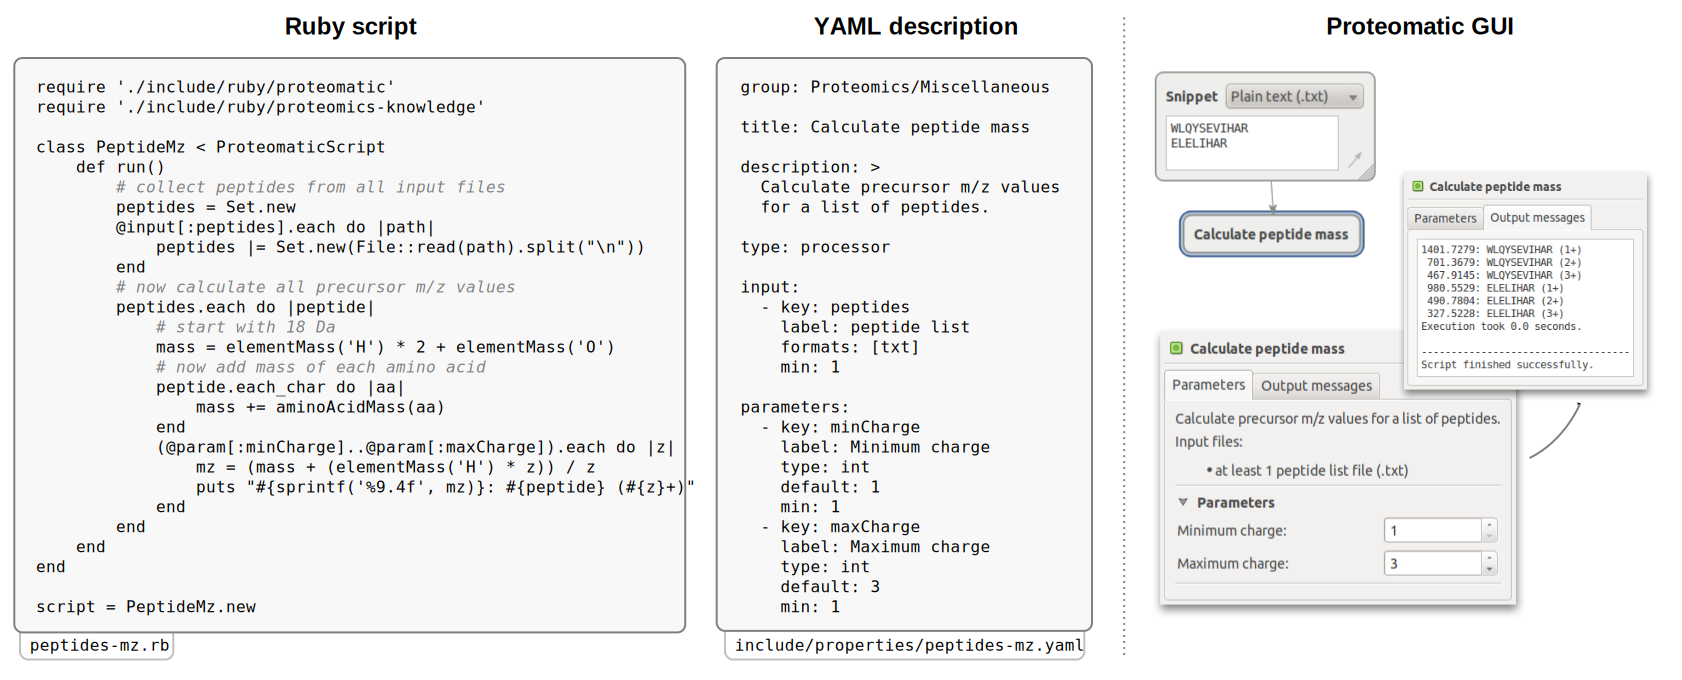
\includegraphics[width=\textwidth]{figures/example-script-2.jpg}
\caption{
{\bf An example of a Proteomatic script.} 
The script, which is implemented in Ruby in this case, is complemented with
a YAML-formatted description which specifies all parameters as well as input
and output files of the script.
The description is used by the Proteomatic front end to automatically construct 
a graphical user interface. This way, prototypes providing novel functionality
or proof of concepts can be deployed early and often.
}
\label{fig:rapid-development}
\end{figure}

\paragraph{File-based data processing.}

One might criticize the apparent lack of visualization capabilities in 
Proteomatic for experimental data and data evaluation results.
This is, however, a design decision which has been made to avoid {\em feature 
creep}, an effect which may lead to failure of software projects due to
an ever-increasing amount of features being implemented which go far beyond the 
originally intended scope.
Proteomatic implements a strictly file-based data processing pipeline which
means that all processing steps are strictly atomic and the output of one
processing step is passed on as one or several files.
This approach allows for manual inspection and intervention at any stage of
a complex pipeline.
Furthermore, all intermediate and final results can be copied to another 
computer or sent via e-mail.
Various standards are emerging for spectral data (mzML, \cite{Deutsch2008}), 
identification results (mzIdentML\footnote{http://www.psidev.info/index.php?q=node/319}), and quantitation results 
(mzQuantML\footnote{http://www.proteomexchange.org/project-organization/workpackages/wp2-standards-development}).
In addition to these standardized file formats, further established file 
formats such as plain text or comma-separated values are used for intermediate 
results.
For each of the file formats employed, specialized viewers already exist
or are currently in development\footnote{http://code.google.com/p/mzidentml-viewer}.
When the user double-clicks on an output file, Proteomatic delegates the
file handling to the underlying operating system which even has a program 
registered to handle the file type or may make a suggestion.
Therefore, a requirement for handling various file types within Proteomatic
is not evident.


% \begin{todo}
% - decentralized system
% - many researches, many computers for data evaluation
% - low impact of failing single computers on overall performance 
% - functional data evaluation setup can be restored in a straightforward way
% - automatic software downloading
% - also beneficial in education
% - two-level design (CLI and GUI) allows for usage in situations which too 
%   complex to be feasible for handling in the GUI
% - rapid deployment of novel functionality
% - support for multiple scripting languages
% 
% outlook:
% - remote execution and the cloud
% - filetracker queries


\section{Automated quantitation of metabolically labeled samples}

One of the studies presented in this thesis provides a comprehensive list of 
experimentally deduced chloroplast proteins for \cre~for the first time
(manuscript 2).
The list of 895 chloroplast-localized proteins has been compiled using
a quantitative approach via spectral counting.
The necessary data evaluation and filtering steps have been implemented
as processing steps in Proteomatic.
In manuscript 3, the list of chloroplast proteins has been manually extended 
to 996 proteins, including chloroplast-encoded proteins and further proteins
which have previously been characterized as localized to the chloroplast.
In addition to experimental localization, the anaerobic response of the 
experimentally deduced chloroplast proteome of the green alga is characterized 
in manuscript 2. 
From 895 proteins, 425 proteins could be quantified in manuscript 2, 
confirming the anaerobic induction of hydrogenase, a protein involved in 
hydrogen production.
Furthermore, induction on the protein level could be confirmed for various 
proteins previously found to be induced on the transcript level,
including proteins involved in fermentative metabolism (see Fig.~\ref{fig:qtrace-mia}).
In addition to many ribosomal proteins with varying levels of induction,
pointing to a re-structuring of the chloroplast metabolism via translational 
regulation, a small set of 23 uncharacterized proteins was found to be induced
and thus represent interesting candidates for further research.

The framework for high-throughput quantitation of metabolically labeled 
samples, in this case by SILAC, is provided by qTrace.
qTrace is a targeted quantitation program which takes a list of peptides
identified via MS/MS, along with their retention time, as input and then 
reconstructs the corresponding isotope envelopes which are subsequently 
matched to the full scans (see Appendix A for a detailed description).
In comparison to MS/MS-based quantitation, this strategy allows for the
incorporation of a large set of data points during the final peptide ratio
estimation because peptides usually elute for a time span long enough to
show their precursor peaks in several successive full scans.
It is obvious that the assignment of precursor peaks in full scans is highly
ambiguous, given the fact that several distinct peptides can yield the
same {\em m/z} values and therefore, peptide identification is not possible
using intact peptide masses only.
In order to remove spurious precursor peak assignments, several filters are 
employed.

\begin{figure}
\includegraphics[width=\textwidth]{figures/fig6.jpg}
\caption{
{\bf Quantitation results for SILAC labeled \cre~samples under anaerobiosis.} 
Black dots denote quantitation results which have been confirmed by an
MS/MS identification within a retention time window of one minute, white dots
denote confirmation via a manual AMT approach.
Graph A shows quantitation results for 345 proteins stemming from multiple 
combinations of peptide, band, and charge. An additional set of 80 proteins 
deduced from only one such combination are depicted in graph B.
}
\label{fig:qtrace-mia}
\end{figure}

\paragraph{Confidence of peak assignments.}

The inherent ambiguity resulting from assigning precursor peaks in full scans
is compensated with the requirement of MS/MS identification in the same band
within a small retention time window of one minute.
The assumption made by such a {\em MS/MS requirement filter} is that once the
identity of a precursor peak has been established via MS/MS, this information
can be expected to remain true within a short time span.
Furthermore, if protein fractionation via SDS-PAGE has been employed, a filter
which determines for each protein the SDS-PAGE band it has been most abundantly
identified in via MS/MS and subsequently discards all quantitation events
from other bands, allowing for a user-defined tolerance, under the assumption
that peak assignments in atypical bands are potential artifacts.

While these filters allow to increase the confidence of quantitation results
by coupling them to the identification results in both retention time and
molecular weight dimensions, assignments of peptides to intact precursor
peaks remains a challenge.
Therefore, quantitation results stemming from the analysis of full scans
should be regarded to provide induced candidate proteins in a discovery-based
experiment and further validation by employing molecular biology techniques
is advisable.

\paragraph{Metabolic labeling strategies.}

\begin{figure}
\includegraphics[width=\textwidth]{figures/qtrace-diagram.jpg}
\caption{
{\bf Quantitation results for \textsuperscript{15}N labeled \cre~samples
    under iron deficiency.} 
    Isolated chloroplast proteins from \cre~cultures grown under 
    iron-deficient (\textsuperscript{14}N) and iron-sufficient
    (\textsuperscript{15}N) conditions were mixed and measured via
    GeLC-MS/MS, using five bands from the gel.
    Using Proteomatic, a set of 2,754 distinct peptides could be identified
    via OMSSA which were subsequently passed to qTrace. 
    After carrying out all filtering steps as described in manuscript 2
    and shifting the quantitation results to the protein level,
    a set of 59 proteins or protein groups could be quantified,
    including many light-harvesting proteins.
    Ratios correspond to \textsuperscript{14}N/\textsuperscript{15}N ratios,
    high values correspond to induction under iron deficiency.
    The data presented in this figure was provided by Ricarda H\"ohner.
}
\label{fig:qtrace-15n}
\end{figure}

qTrace supports a variety of metabolic labeling strategies by allowing the 
user to define a non-natural isotope distribution for every chemical element 
occuring in amino acids (hydrogen, carbon, nitrogen, oxygen, and sulfur).
In addition, these non-natural isotope distributions can be applied 
to a restricted set of amino acids.
Using the user-specified label definition, qTrace is able to handle a variety
of labeling strategies, including SILAC, \textsuperscript{15}N labeling (see 
Fig. \ref{fig:qtrace-15n}), or \textsuperscript{18}O labeling 
\citep{Miyagi2007}.
\textsuperscript{13}C Arg SILAC labeling typically introduces a mass shift
of 6 Da between two sister peptides if trypsin is used for enzymatic digestion
because at most one arginine residue is typically expected per peptide and
arginine contains 6 carbon atoms.
Quantitation results stemming from \textsuperscript{15}N labeled samples
can be regarded as more confident because the mass shift between sister peptides
depends on the amino acid composition.
This is because the label is introduced into every amino acid, and the number of
nitrogen atoms is varying between different amino acids.

\paragraph{Induction of unannotated proteins.}

The large-scale quantitation approach presented in manuscript 2 resulted
in a handful of proteins of unknown function shown to be induced under
anaerobiosis.
The quantitative results for these proteins hint towards a possible role
in response to the experimental condition.
Therefore, such proteins present interesting candidates for further research.

\section{Further analysis of the \cre~chloroplast proteome}

\begin{figure}
\includegraphics[width=\textwidth]{figures/all-four-charts.jpg}
\caption{
}
\label{fig:mia-review-isolines}
\end{figure}

\begin{figure}
\includegraphics[width=\textwidth]{figures/wheel-yet-again-oh-noes.jpg}
\caption{
}
\label{fig:mia-review-wheel}
\end{figure}

\section{Proteogenomic genome annotation}

Manuscript 4 introduces a new version of the Genomic Peptide Finder and
presents a high-throughput strategy for the statistical validation of
GPF peptides and their subsequent use in a proteogenomic genome annotation
approach using AUGUSTUS.

The new GPF version implements two major features:

\begin{enumerate}
\item {\bf Intron splits may occur within a single coding nucleotide triplet.}
This addition increases search sensitivity by considering a possible intron
split in three locations per nucleotide triplet instead of one.

\item {\bf Splice donor/acceptor site consensus sequences may be specified.} 
This modification increases search specificity because spliced peptides with
unusual splice donor/acceptor sites are omitted from the results.
\end{enumerate}

Most importantly, the search has been greatly accelerated due to the use
of a one-time pre-processing step in which an index of the genomic DNA sequence
to be used is created.
For \cre, this indexing step produces an index file of 2.4 GiB in about 15 
minutes.
This initial cost is later compensated during the search which performs
20 queries per second on average on commodity hardware, using commodity flash 
memory to store the index file for faster random access.

Apart from these technical improvements, a method for the automated validation 
of GPF candidate peptides, employing standard database search programs such as 
OMSSA was established.
This allows for statistically robust identification of GPF-deduced peptides
alongside gene model peptides.
Furthermore, an annotation pipeline was established in which resulting GPF
peptides are passed to AUGUSTUS, which performs an {\em ab initio} gene 
model prediction supplemented by various extrinsic hint sources including
GPF peptides.
It is therefore a major contribution of this thesis that an automated
proteogenomic annotation of the \cre~genome in which MS/MS data generated
for various unrelated purposes can be re-used for the generation of
extrinsic AUGUSTUS hints is available.

Using measurements of 949 bands which have been made in various experiments,
a set of 9,336 statistically significant peptides could be deduced via 
{\em de novo} prediction and subsequent GPF processing.
From this peptide set, 1,318 peptides (14\%) contained an intron split,
324 of which were spliced within a single coding nucleotide triplet,
amounting to 25\% of all spliced peptides.
The na\"ive assumption that the consideration of triplet-spliced peptides
would enhance the overall number of spliced peptides by a factor of three,
which would correspond to a relative triplet-spliced peptide amount of 66\%
is therefore not met.
This is in line with previous results which estimate the relative amount
of triplet splicing to be surprisingly low at around 45\% in plants 
\citep{Tomita1996}.

\begin{figure}
\includegraphics[width=0.8\textwidth]{figures/gpf-omssa.jpg}
\caption{
{\bf Validation of GPF candidate peptides via a target/decoy approach
    using previously established gene models.} 
    Statistical significance of identified GPF candidate peptides is 
    assessed by employing a target/decoy approach with existing gene models 
    which may be incomplete but can be expected to contain a high amount of 
    correct sequences.
    GPF peptides are also added to the candidate peptide pool, and the database
    search program (OMSSA) assigns the best match from the pool to each
    MS/MS spectrum, resulting in comparable E-values in between the two
    peptide sources.
    The final E-value threshold determination is performed under exclusive
    consideration of the gene model target and decoy peptides.
    The determined threshold is then applied to all peptide/spectral matches,
    including those to GPF peptides.
}
\label{fig:gpf-omssa}
\end{figure}

The presented pipeline for the generation of peptide hints for the purpose of
proteogenomic annotation is similar to the exon splice graph approach proposed
by \citeauthor{Tanner2007} in that it uses MS/MS scans as a source of candidate
peptides.
However, the GPF approach is less biased in comparison to the exon splice graph
approach because it does not require exon/intron prediction as a first step.
GPF candidate peptides are solely generated from MS/MS {\em de novo} sequencing
and subsequent mapping of the resulting peptides to the genome, using a 
user-defined maximum intron length and a set of possible splice donor/acceptor 
site consensus sequences.
This means that intron prediction is carried out on a per-peptide basis, and
all peptides are treated independently.
The actual validation of extrinsic hints and splice site detection is
carried out by AUGUSTUS in the final annotation step.
Moreover, the approach is highly flexible because no specialized database
search program is required because candidate peptides are inferred by GPF
and then passed down the evaluation pipeline alongside a protein database
(see Fig.~\ref{fig:gpf-omssa}).

% \paragraph{Improved GPF performace.}

Although a gene model protein database is used to estimate the FDR of peptide 
identifications, the final GPF-deduced peptides which are exported as
peptide hints do not originate from this database, although in the case
of \cre, a large portion of these gene model peptides could be 
independently confirmed via the combination of {\em de novo} sequencing and 
GPF (see manuscript 4).
The high amount of 53\% confirmed gene model peptides points to a improvement 
of sensitivity of the new GPF version.
One might argue that the use of {\em de novo} prediction, followed by
error-tolerant, intron-aware matching to a genomic sequence is prone to
produce large sets of similar peptides.
However, this is not the case.
The 10 peptides which are generated by PEAKS for every MS/MS scan are 
reduced to 3.4 peptides on average after employment of GPF.
Furthermore, as has been shown in manuscript 4, 97\% of all GPF-deduced 
peptides are incorporated into the final gene models by AUGUSTUS.
Because several other hint sources were available to AUGUSTUS and none of
these sources is trusted unconditionally, these numbers suggest a strong 
specificity of GPF peptides.

\section{Identification of novel targets}

A combination of qTrace and the Genomic Peptide Finder can produce especially
interesting results.
As shown in manuscript 4, the Genomic Peptide Finder can confirm a substantial
amount of gene model peptides.
In addition, previously unknown peptides may result from the analysis.
This is especially true for organisms which for which genome sequencing and
genome annotation are unavailable or are still in the early stages.
Mass spectrometric data stemming from such organisms can be expected to
yield a high amount of novel peptides.
These peptides can be passed to qTrace along with identified gene model 
peptides, possibly resulting in the identification of induced peptides which
are not part of a gene model.
If there is a peptide A stemming from already existing, possibly preliminary gene
models, and a peptide B which has been identified via GPF only, and both
are shown to be co-regulated via qTrace, it might be that the gene model
containg A must be modified to also include B, if B is in close proximity to A
on the genome (and the direction of the reading frames of A and B is equal).
Quantitative information, mapped to the genome, might also be useful to
support proteogenomic genome annotation because peptide clusters exhibiting 
similar regulation patterns might be part of the same gene.
Furthermore, the confidence of a gene model-independent deduction of a novel 
GPF peptide is increased if the same peptide could also be quantified in full
scans, preferably via \textsuperscript{15}N labeling in which the individual
mass shift introduced by the peptide-dependent number of nitrogen atoms acts
as signature fingerprint for the peptide.
Although this mass shift does not confirm the amino acid sequence of the 
peptide, it represents a strong hint that the number of nitrogen atoms in
the GPF peptide is correct.

\section{Outlook}

Although the presented software systems are fully functional and have been
shown to provide useful results in the various studies, there are many
points which should be addressed in the future to further improve the software.

\subsection{Proteomatic}

\paragraph{Remote execution.}

In comparison to a web browser-based user interface as provided by TPP, the 
GUI provided by Proteomatic can be regarded as highly accessible due to 
the support for {\em drag and drop} operations and an overall look and feel
which matches the underlying operating system.
Also, the decentralized approach implemented by Proteomatic leads to a
higher responsiveness of the system because network communication is not 
involved in the pipeline creation process and there is no central server which
could be overloaded from too many requests.
However, it would be favorable to have the option to send a pipeline to a 
dedicated server which would then execute the pipeline and leave the 
user's computer responsive.
In such a setup, the decentralized data evaluation approach would be 
supplemented with an optional centralized data processing step which can
aid in data evaluation but is not vital for the overall availability of
data evaluation functionality.
Because the scripts back end of Proteomatic is able to automatically resolve 
external software dependencies, this approach seems especially feasible because
the server could mimick the specific environment of the user as defined by
the version number currently installed on the user's computer.

\paragraph{Incorporation of a freely available {\em de novo} sequencing software.}

While protein identification and quantitation is implemented in Proteomatic
using free software, the proteogenomic pipeline approach presented in 
manuscript 4 depends on PEAKS for the generation of {\em de novo} predictions.
GPF does not require completely sequences peptides but also works with
short sequence tags that have defined N- and C-terminal masses.
Existing free alternatives such as Lutefisk \citep{Johnson2002}, PepNovo 
\citep{Frank2005} and CompNovo \citep{Bertsch2009} should be evaluated in
terms of performance.
This can be easily accomplished by replacing the {\em de novo} prediction
step with each software, re-running the entire annotation pipeline and 
determining the amount of resulting GPF peptides that have been successfully
incorporated into the resulting gene models.
Once such a freely available {\em de novo} prediction software has been
incorporated, the proteogenomic genome annotation approach could be 
established in a distributed manner which yields comprehensive peptide hints.

\paragraph{Centrally maintained repository of data files.}

The strategy to collect information about external software and offer the
use of these programs by means of a hierarchical menu of processing steps
could be extended to data files such as genome and protein databases.
By providing a centrally maintained repository containing links to freely
available data files in addition to freely available software, the entire
data evaluation process would be simplified because the user is not
required to search for the appropriate files on the internet.
Like software is downloaded automatically as soon as it is required for the 
first time, data files could be downloaded when they are required and would
then remain on the user's computer until a newer version is published in
the Proteomatic data repository.

\paragraph{Refinement of workflow interaction metaphors.}

Proteomatic currently provides a way to establish complex file-based data 
evaluation workflows which can be expressed by a directed acyclic graph (DAG),
iteratively executing processing steps for which all input requirements are
met and thus eventually resolving the entire pipeline.
Software developers are used to the possibility to create loops in their
workflows which is especially useful if the same task should be repeated
several times on different input files.
In order to provide this mechanism to users, Proteomatic offers an interaction 
metaphor which turns a {\em file list} into a {\em file batch}, denoted by a 
yellow arrow (see Fig.~\ref{fig:appendix-b-pipeline} for an example).
However, as can be seen in the final processing steps of 
Fig.~\ref{fig:appendix-b-pipeline}, this mechanism complicates matters when
a set of input files should be used as a batch in one situation, and as a
plain list in another situtation.
Currently, this can only by achieved by turning the file batch into a file
list by inserting two CSV file merging steps.
If these steps would be ommited and the original CSV results file batch
would be provided as input to the {\em Generate AUGUSTUS hints} processing
step, 46 output files with partially redundant entries would emerge from
the pipeline.
A possible solution to this issue would be to define batch behaviour per
arrow instead, thus allowing a set of files to be used as input to one single 
processing step yielding a single output file, but at the same time the
set of files could be used for the repeated execution of another processing
step, yielding one output file for every specified input file.


\paragraph{Filetracker querying.}

\subsection{qTrace}

\paragraph{Performance comparison to existing alternatives.}

\paragraph{Untargeted quantitation.}

\subsection{Genomic Peptide Finder}

\paragraph{Increased search sensitivity.}

\paragraph{Processing of large genomes.}

% outlook:
% - also provide data, not just tools
% - remote execution (but local creation)
% - refinement of the workflow interaction metaphors (batches should be defined
%   per arrow, not per input file box)
% \end{todo}


% \cleardoublepage
\cleardoublepage
% ==============================================================
\chapter{Summary}
% ==============================================================

A novel platform for the evaluation of mass spectrometric data has been
established and was subsequently employed for the evaluation of measurements
performed to characterize the chloroplast proteome of \cre~and elucidate
the anaerobic response of the chloroplast proteome.
Proteomatic provides user-friendly access to mass spectrometric data 
evaluation programs and allows for the construction of complex workflows.

In order to facilitate the large-scale characterization of the chloroplast
proteome, qTrace has been designed to automate the peptide and protein 
quantitation process in full scans.
qTrace supports a variety of metabolic labeling strategies and has 
led to the confirmation of chloroplast protein induction under anaerobiosis
as well as the identification of several proteins of unknown function
which represent potential targets for further research.

{\em De novo}-based peptide sequencing is a powerful approach for the annotation
of MS/MS spectra, complementing gene model-based data search algorithms.
The inherent ambiguity of {\em de novo} sequenced peptides is greatly diminished
by the Genomic Peptide Finder which correlates the potentially erroneous
peptide sequences to the genomic DNA sequence of an organism, thereby discarding
spurious peptides and correcting ambiguous sequences.
An improved version of the Genomic Peptide Finder regarding sensitivity, 
specificity, and search speed, has been presented in this thesis.

Furhermore, a method for the automated statistical validation of GPF peptides
has been developed and has led to the possibility of using GPF peptides as
an extrinsic hint source for AUGUSTUS in a proteogenomic genome annotation 
approach.

All software developed in the scope of this thesis is publicly available
at \href{http://github.com/specht}{http://github.com/specht}.


% \cleardoublepage
% ==============================================================
\chapter*{Appendix A: qTrace - Rapid quantitation of metabolically labeled sister peptides}
\markboth{Appendix A: qTrace - Rapid quantitation of metabolically labeled sister peptides}{Appendix A: qTrace - Rapid quantitation of metabolically labeled sister peptides}
\addcontentsline{toc}{chapter}{Appendix A: qTrace - Rapid quantitation of metabolically labeled sister peptides}
% ==============================================================

\begin{figure}[h]
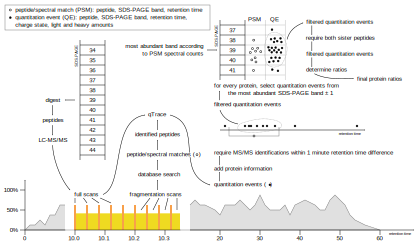
\includegraphics[width=\textwidth]{figures/exp-setup.jpg}
\caption{
{\bf Caption.} 
Caption here.
}
\label{fig:qtrace-workflow}
\end{figure}



% \cleardoublepage
% ==============================================================
\chapter*{Appendix B: Proteomatic workflow for proteogenomic genome annotation}
\markboth{Appendix B: Proteomatic workflow for proteogenomic genome annotation}{Appendix B: Proteomatic workflow for proteogenomic genome annotation}
\addcontentsline{toc}{chapter}{Appendix B: Proteomatic workflow for proteogenomic genome annotation}
% ==============================================================

% ==============================================================
\renewcommand{\baselinestretch}{1.0} 
\renewcommand{\arraystretch}{1.0} 
% ==============================================================


\newpage
\bibliography{library}
\addcontentsline{toc}{chapter}{References}
\markboth{References}{References}
% \bibliographystyle{abbrvnat-no-url}
\bibliographystyle{bst}
    
\cleardoublepage
% ==============================================================
\chapter*{Acknowledgements}
\markboth{Acknowledgements}{Acknowledgements}
\addcontentsline{toc}{chapter}{Acknowledgements}
% ==============================================================

First of all, I would like to thank Michael Hippler

I would also like to thank my wife, Jule, who comes up with splendid ideads
which tend to work out.

\cleardoublepage
% ==============================================================
\chapter*{Curriculum vitae}
\markboth{Curriculum vitae}{Curriculum vitae}
\addcontentsline{toc}{chapter}{Curriculum vitae}
% ==============================================================

% Michael Specht \\
% Toppheideweg 34 \\
% 48161 Münster
% 
% Phone: +49 251 4808158 \\
% E-mail: \href{mailto:michael.specht@uni-muenster.de}{michael.specht@uni-muenster.de}
% 

\begin{longtable}{@{}lp{12.5cm}}

\cvsubheader{Personal details}

Date of birth: & December 23, 1981 \\
Place of birth: & Magdeburg, Germany \\
Marital status: & married, two children\\
\\

\cvsubheader{Publications}

04/2011 & Terashima M., {\bf Specht M.}, Hippler M. (2011). The chloroplast proteome: A survey from the {\em Chlamydomonas reinhardtii} perspective with a focus on distinctive features. Current Genetics 2011 (in press). \\%; DOI: \href{http://dx.doi.org/}{} (in press). \\

03/2011 & {\bf Specht M.}, Stanke M., Terashima M., Naumann-Busch B., Janßen I., Höhner R., Hom E. F. Y., Liang C., Hippler M. (2011). Concerted action of the new Genomic Peptide Finder and AUGUSTUS allows for automated proteogenomic annotation of the Chlamydomonas reinhardtii genome. Proteomics 2011; doi: \href{http://dx.doi.org/10.1002/pmic.201000621}{10.1002/pmic.201000621} (in press). \\

02/2011 & {\bf Specht M.}, Kuhlgert S., Fufezan C., Hippler M. (2011). Proteomics to go: Proteomatic enables the user-friendly creation of versatile MS/MS data evaluation workflows. Bioinformatics (2011) 27 (8): 1183-1184; doi: \href{http://dx.doi.org/10.1093/bioinformatics/btr081}{10.1093/bioinformatics/btr081}. \\

07/2010 & Terashima M., {\bf Specht M.}, Naumann B., Hippler M. (2010). Characterizing the anaerobic response of Chlamydomonas reinhardtii by quantitative proteomics. Mol Cell Proteomics, 9(7), 2010: 1514-32; doi: \href{http://dx.doi.org/10.1074/mcp.M900421-MCP200}{10.1074/mcp.M900421-MCP200}. \\

08/2009 & Fufezan C., {\bf Specht M.} (2009). p3d – Python module for structural bioinformatics. BMC Bioinformatics (2009) 10:258; doi: \href{http://dx.doi.org/10.1186/1471-2105-10-258}{10.1186/1471-2105-10-258}. \\

11/2007 & Ropinski T., {\bf Specht M.}, Meyer-Spradow J., Hinrichs K., Preim B. (2007). Surface Glyphs for Visualizing Multimodal Volume Data. Vision, Modelling and Visualization (VMV) (3-13), Saarbrücken, 2007. \\

% \newpage 

\cvsubheader{Talks}

\cvtitle{03/2011}{DGMS 2011, Dortmund}
& Proteomics to go: Proteomatic enables the user-friendly creation of versatile MS/MS data evaluation workflows. \\
\tabspace\\


\cvsubheader{Professional experience}

\cvtitle{since 04/2007}{Institute of Plant Biology and Biotechnology\newline Westfälische Wilhelms-Universität Münster}
& Doctoral student in the lab of Prof. Dr. Michael Hippler \newline
% \vspace{6pt}
\vspace{-9pt}
\begin{compactitem}
\item Proteomatic: design and implementation of a user-friendly, decentralized MS/MS data 
evaluation platform \vspace{4pt}\newline
Link: \href{http://www.proteomatic.org}{http://www.proteomatic.org}
% \vspace{-12pt}
% \begin{compactitem}
\item Genomic Peptide Finder: Software for the alignment of MS/MS {\em de novo}
predicted amino acid sequences to the genomic DNA sequence of an organism.
Resulting peptides may be used for evidence-based proteogenomic genome annotation. \vspace{4pt}\newline
Link: \href{http://github.com/specht/gpf}{http://github.com/specht/gpf}.
\item qTrace: Software for the high-throughput quantitation of metabolically
labeled samples (e.g. $^{\textrm{13}}$C Arg SILAC or $^{\textrm{15}}$N) in survey scans.\vspace{4pt}\newline
Link: \href{http://github.com/specht/qtrace}{http://github.com/specht/qtrace}
% \end{compactitem}
\item establishment of free MS/MS data evaluation software in the lab, resulting 
in increased throughput, lower costs and proliferation of MS/MS data 
evaluation-related expertise
\end{compactitem}
% \vspace{-6pt}
\tabspace\\

\cvtitle{10/2006 -- 03/2007}{PROVISIO Software GmbH Münster}
& Software developer -- Realtime Rendering Group \newline
\vspace{-9pt}
\begin{compactitem}
\item design and implementation of a fast JPEG decoder
\item implementation of various user interface widgets for Pictomio
(photo viewer software)
\end{compactitem}
\vspace{-6pt}
\tabspace\\

\cvtitle{07/2005 -- 02/2006}{1komma6 Multimediale Dienstleistungen GmbH Münster}
& Internship -- Web development, focus on accessibility \newline
\tabspace\\

% \newpage

\cvsubheader{Education}
\cvtitle{03/2006 -- 11/2006}{Diploma thesis}
& \emph{Glyph-enhanced Volume Visualization}. \newline
Development of a visualization method for the interactive, simultaneous display 
of multiple, related medical data sets (CT and PET).\tabspace\\
% % \input{../../common-en/chromacoding}
% % \input{../../common-en/studienarbeit}
% 

\cvtitle{10/2001 -- 11/2006}{Study of Computational Visualistics}
& Study of Computational Visualistics (computer science with a focus on computer 
graphics) at the Otto-von-Guericke-Universität Magdeburg.\tabspace\\

\cvtitle{09/2000 -- 07/2001}{Alternative civilian service}
& Civilian service at the retirement home "`Luisenhaus"', Potsdam. \tabspace\\

\cvtitle{09/1992 -- 05/2000}{Secondary school}
& Werner-von-Siemens-Gymnasium, Magdeburg. \tabspace\\

% 
% \newpage
% 
\cvsubheader{Further education}
% 
\cvtitle{10/2010}{Advanced Scientific Programming in Python}
& Participated in an autumn school, held in Trento, Italy,
organized by G-Node, the center for Mind/Brian Sciences, and Fondazione Bruno Kessler.\tabspace\\

\newpage

% \cvsubheader{Miscellaneous projects}
% % 
% % % \input{../../common-en/nprflow}
% % % \input{../../common-en/hamster}
% % % \input{../../common-en/tutorium}
% % % \input{../../common-en/vib}
% 
% \cvtitle{02/2003}{Student anti war group}
% & Foundation of the student anti war group at the University of Magdeburg,
% shortly before the beginning of the Iraq war in March 2003.
% Planning and organization of discussion rounds and movie nights. \tabspace\\
% 
% \cvtitle{11/2002 -- 11/2003}{Short film "`pixelle ma belle \#01"'}
% & \begin{compactitem}
% \vspace{-9pt} 
% \item design and implementation of a distributed video rendering software
% \item development of an alternative, low-cost blue screen method
% \end{compactitem}
% \vspace{6pt} 
% Link: \href{http://www.pixellemabelle.de}{www.pixellemabelle.de}
% \tabspace\\
% 
% % % \input{../../common-en/fx}
% % % \input{../../common-en/ferienlager}
% % % \input{../../common-en/zeitnahme}
% % 
% \cvsubheader{Skills}
% % 
% 
% foreign languages
% & English (fluent)\newline
% French (basic knowlegde) \tabspace\\
% 
% programming
% & C, C+\kern-0.2em +, Qt, Ruby, Python, PHP, Java, Assembler, XHTML, CSS, Ajax, MySQL\tabspace\\
% 
% software
% & Linux, Windows, Mac OS X \newline
% GIMP, Inkscape, OpenOffice, \LaTeX
% Git, Subversion, CSV\tabspace\\

% 
\end{longtable}
% 



\end{document}
